\documentclass[slidetop, mathserif]{beamer}

% \mode<presentation>
% {
% 	\usetheme{Warsaw}
% 	\setbeamercovered{transparent}
% }

% \usepackage{caption}
\usepackage{subcaption}
\captionsetup{compatibility=false}


\mode<presentation>{
	\usetheme{Berlin}
	\setbeamercovered{transparent}
	\usefonttheme{professionalfonts}
}

\usepackage{amsmath, amsfonts, amssymb}
\usepackage{mathrsfs,dsfont}

\newcommand{\norm}[1]{\left\|#1\right\|}
\newcommand{\suchthat}{-\hspace{-10pt}\ni\hspace{-10pt}-}


\AtBeginSection[]
{
   \begin{frame}
       \tableofcontents[currentsection]
   \end{frame}
}

\addtobeamertemplate{navigation symbols}{}{%
    \usebeamerfont{footline}%
    \usebeamercolor[fg]{footline}%
    \hspace{1em}%
    \insertframenumber/\inserttotalframenumber
}

%% want to use verbatim: \begin{frame}[fragile]

\title[Metrics for Tracking]{Metrics for Trackings: Evaluations and Comparisons}
\author[chy1010]{Chien, Hung-Yu (chy1010) \\ {\tt andy1010@gmail.com}}
\date{\today}

\begin{document}

\frame{\titlepage}

\section[Outline]{}
\begin{frame}
	\frametitle{Outlines}
	\tableofcontents
\end{frame}

\section{Matchings and Associations}

\begin{frame}
	\frametitle{MOT (Multiple Object Tracking)}
			
	Given a video, the task of MOT consists of 
	\begin{itemize}
		\item locating multiple objects,
		\item maintaining their identities, and
		\item yielding their individual trajectories.
	\end{itemize}
			
	In more details, \emph{each object is assigned a unique id in a frame.}
	And \emph{objects with the same id in consecutive frames form a trajectory}.
			
	\begin{figure}
		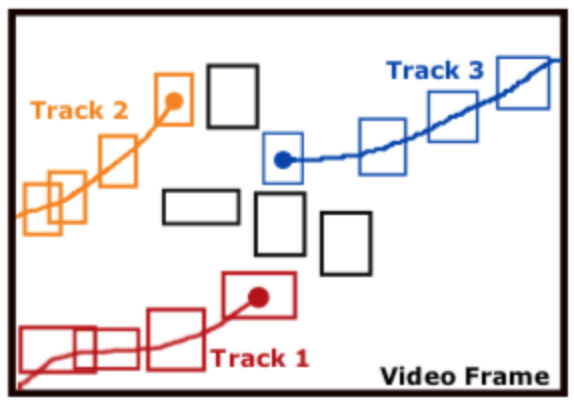
\includegraphics[height=70pt]{pics/fig1.png}
		\caption{Objects with the same id from different frames form trajectories.}
	\end{figure}
			
\end{frame}

\begin{frame}
	\frametitle{Matching / Association in Different Levels}
			
	% Whatever how we perform trackings,
	% new nominal ids are assigned to detected objects in every frames.
	% Hence to compare the results, we need to match the new ids
	% with the original ids.
	To compare the results, we need to match the new ids
	with the original ids.
		
	\vspace{4pt}
			
	The matchings are done in different levels such as:
	\begin{itemize}
		\item {\bf framewisely / detection levels}:
		      match ground-truth objects (denoted by gtDets)
		      with predictions (denoted by prDets) frame by frame.
		\item {\bf sequentially / trajectory levels}:
		      match each ground-truth id to an hypothesis id along a sequence of frames.
		\item {\bf associations of trajectories}:
		      associate ground-truth ids with several non-overlapping preditive trajectories.
	\end{itemize}
		
	% To give some partial credits to some peices of trajectories,
	% we may also associate the ground-truth ids with preditive ids (not 1-1 relation).
			
\end{frame}

\begin{frame}
	\frametitle{Trivial Notions}
			
	\begin{itemize}
		\item Denote $F:=\{f_0, f_1, \ldots, f_{N-1}\}$ as the set of frames.
		\item If $\Pi$ is a framewise matching, it can be a matching in a frame $f$ and specified by $\Pi^{(f)}$;
		      or be a matching during all frames.
		\item When $\Pi$ denotes a global matching, it is the union of all its sections:
		      $\Pi = \cup_{f\in F}\Pi^{(f)}$.
		\item Furthermore, once a collection $E$ is well-defined in each frame,
		      we denote $E^{(f)}$ as the $f$-section, i.e. elements in frame $f$.
		      		      		      
	\end{itemize}
			
	For a ground-truths $g$ or a prediction $p$, denote
	\begin{itemize}
		\item $f_g$ / $f_p$ as the frame it appears;
		\item $\text{gtId}(g)$ / $\text{prId}(p)$ as its id;
		\item $\text{gtTr}(g)$ / $\text{prTr}(p)$ as its trajectory (objects with the same id).
	\end{itemize}
\end{frame}

\subsection{Matching in Detection Levels}

\begin{frame}
	\frametitle{Matching in Detection Levels}
			
	% To perform matching, similarity scores of any ground-truth and any prediction
	% are defined. For example, IoU and $\max\{1-\text{dist}, 0\}$ are often used,
	% where dist is the central distance.
	In detection levels, scoring functions such as $\max\{1-\text{dist}, 0\}$ and IoU
	are often used to measure similarities, where dist is the central distance.
			
	\begin{figure}
		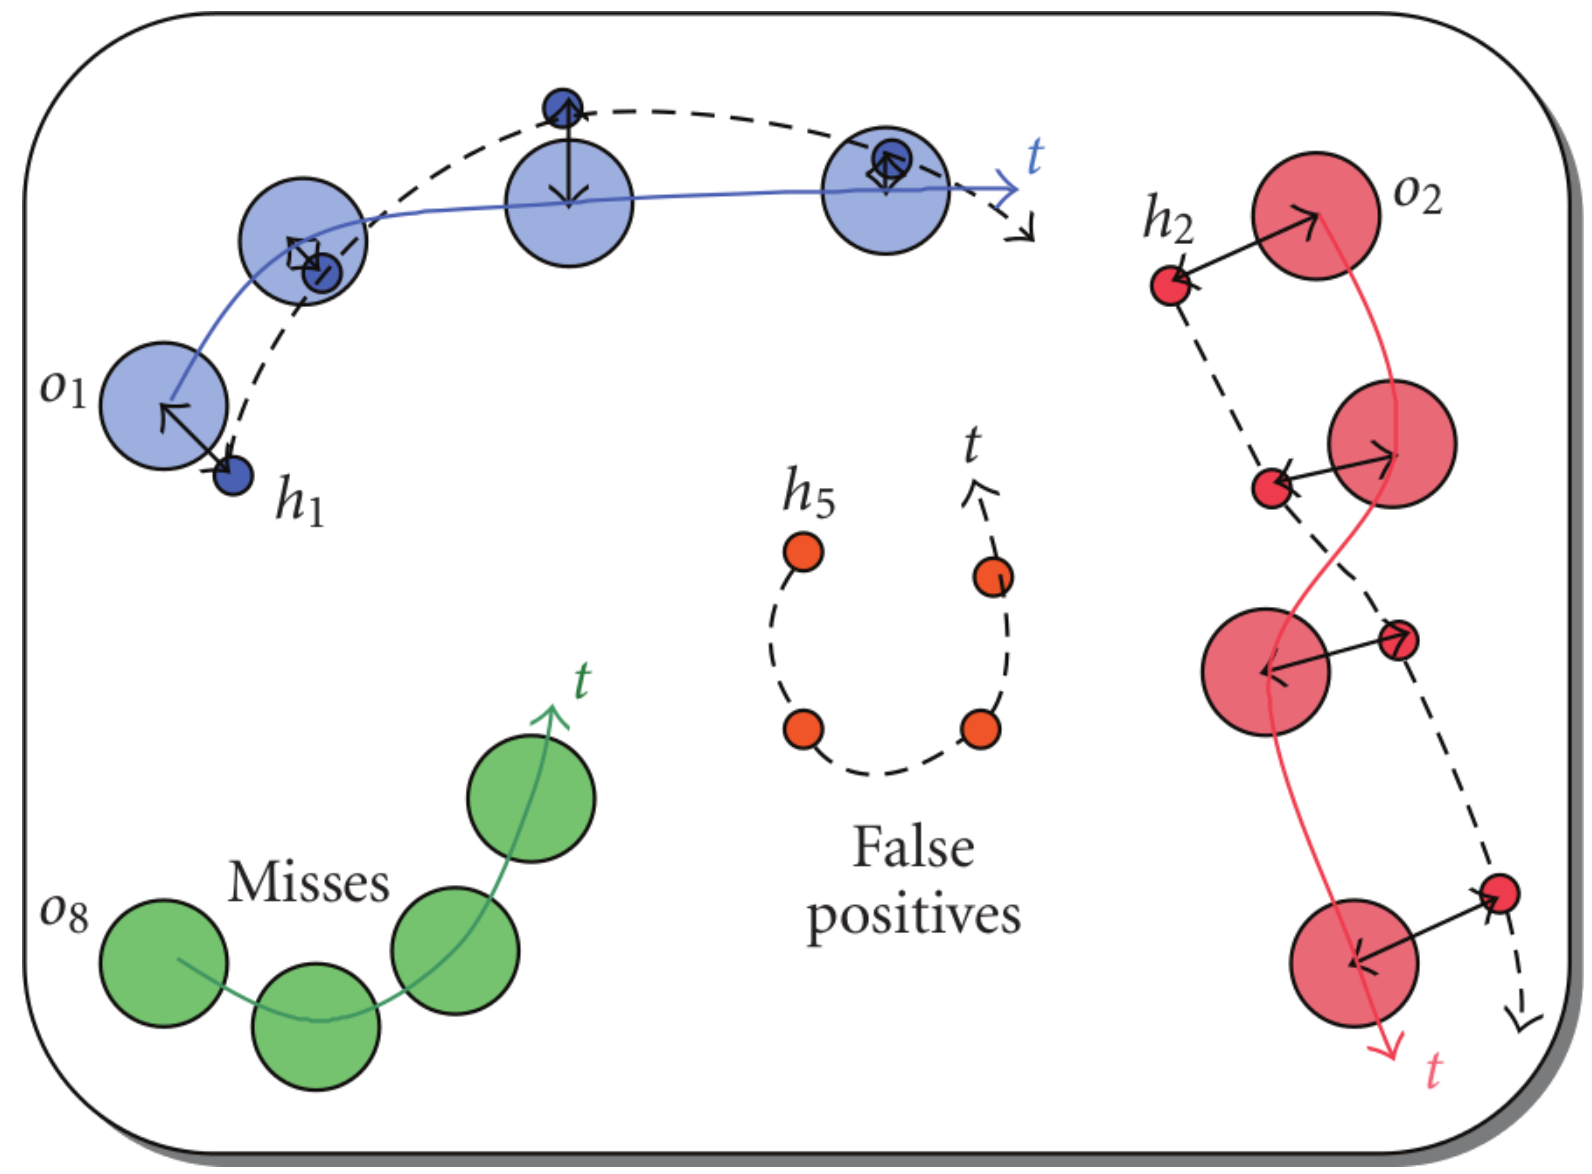
\includegraphics[width=120pt]{pics/fig2.png}
		\caption{Matchings, false positives and misses in consecutive frames.
		Here the similarity is measured by the central distances.}
	\end{figure}
			
\end{frame}

\begin{frame}
	\frametitle{Similarity Threshold and the Quantities TP, FN and FP}
		
	Denote the similarity function by $\mathcal S$.
	To filter out bad matches, we may set a threshold $\alpha$.
	Once a matching $\Pi_\alpha$ under threshold $\alpha$ is done, it satisfies
	\[
		\forall\ (g,p)\in\Pi_\alpha, ~ \mathcal S(g,p) \geq \alpha.
	\]
	Then we can define the quantities TP, FN, FP in detection levels.
	\begin{itemize}
		\item TP: matched pairs in a matching $\Pi_\alpha$.
		\item FP: non-matched predictions.
		\item FN: non-matched ground-truths.
	\end{itemize}
	Remark: there may be several matchings fulfilling the similarity threshold.
\end{frame}


\begin{frame}
	\frametitle{IDSW in Consecutive Frames}
			
	An {\bf IDSW (id switch)} event means there exist TP pairs, say $(g_i, p_j)\in\Pi^{(f)}$,
	$(g_k, p_\ell)\in\Pi^{(f+1)}$, in two consecutive frames
	$f$ and $f+1$ that satisfy
	\[
		\text{gtId}(g_i) = \text{gtId}(g_k),\ 
		\text{prId}(p_j) \neq \text{gtId}(p_\ell).
	\]
	Actually, this is an \emph{id mismatch} occuring in frame $f+1$.
	If two objects exchange their ids in new frame, then this is regarded as $2$
	IDSW events.
	\begin{figure}
		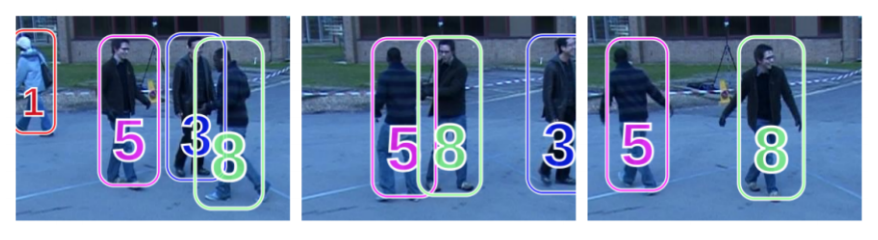
\includegraphics[width=180pt]{pics/fig3.png}
		\caption{The ids 3 \& 8 exchanges. 2 IDSW events.}
	\end{figure}
			    
\end{frame}

\subsection{Matching in Trajectory Levels}

\begin{frame}
	\frametitle{Matching in Trajectory Levels}
			    
	% Matchings here are done by associating one ground-truth trajectory
	% % ({\tt gtTraj})
	% to one predictive trajectory.
	% % ({\tt prTraj})
	% Denote such matchings by swash fonts $\mathfrak P$.
		
	Matchings here are constructing 1-1 relation between ground-truth ids and preditive ids.
			    
	\quad
			
	% The similarity of a {\tt grTraj} and a {\tt prTraj} is often divided into
	% different levels: `mostly tracked' and `mostly lost'.
	Note that \emph{the similarities of two trajectories still depend on the
	framewise matching under some threshold.}
	% Here it is usually defined in a Jaccard index (IoU) way:
	% \[
	%     \mathcal S_{\rm tr}(\text{\scriptsize gtTraj}, \text{\scriptsize prTraj}, \Pi_\alpha) =
	%         |\text{TP}| / (|\text{TP}|+|\text{FN}|+|\text{FP}|).
	% \]
	\begin{figure}
		\begin{subfigure}{.5\textwidth}
			\centering
			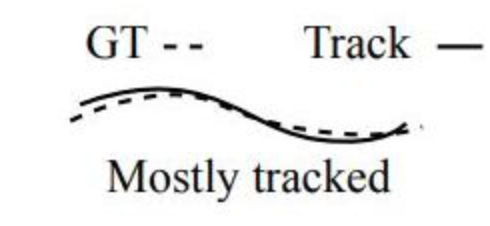
\includegraphics[width=100pt]{pics/fig4.png}
		\end{subfigure}%
		\begin{subfigure}{.5\textwidth}
			\centering
			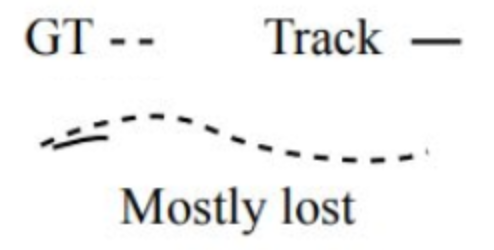
\includegraphics[width=90pt]{pics/fig5.png}
		\end{subfigure}
		\caption{Mostly tracked \& mostly lost.}
	\end{figure}
			
\end{frame}


\begin{frame}
	\frametitle{Similarity of Trajectories}
			
	Similarity scores here are measured
	by counting overlapping and the rest parts of each pair of trajectories.
			
	\vspace{5pt}
			
	Let $\mathfrak g$, $\mathfrak p$ be a pair
	and $\alpha$ be a (detection-) similarity threhold.
	We can also define the analogues:
	\begin{itemize}
		\item $\mathcal{TP}$, $\mathcal{TP}_{\mathfrak g, \mathfrak p}$:
		      the overlapping part of $\mathfrak g$ and $\mathfrak p$.
		      \[
		      	\mathcal{TP} := \{(g,p)\ |\ 
		      	g\in\mathfrak g,~
		      	p\in\mathfrak p,~
		      	f_g=f_p,~ \mathcal S(g,p)\geq \alpha\}
		      \]
		\item $\mathcal{FP}$, $\mathcal{FP}_{\mathfrak g, \mathfrak p}$:
		      the non-matched predictions.
		      \begin{align*}
		      	\mathcal{FP} := & \{ p\in\mathfrak p\ |\ 
		      	\nexists\ g\in\mathfrak g ~\suchthat~ \mathcal S(g,p)\geq\alpha,~ f_g=f_p.\}
		      \end{align*}
	\end{itemize}
			
\end{frame}

\begin{frame}
	\frametitle{Similarity of Trajectories}
			
	\begin{itemize}
		\item $\mathcal{FN}$, $\mathcal{FN}_{\mathfrak g, \mathfrak p}$: the non-matched ground-truth objects.
		      \begin{align*}
		      	\mathcal{FN} := & \{ g\in\mathfrak g\ |\ 
		      	\nexists\ p\in\mathfrak p ~\suchthat~ \mathcal S(g,p)\geq\alpha,~ f_p=f_g.\}
		      \end{align*}
	\end{itemize}
			
	The similarity of trajectories is defined by
	\[
		\mathcal S_{\rm tr}(\mathfrak g, \mathfrak p) :=
		\dfrac{|\mathcal{TP}_{\mathfrak g,\mathfrak p}|}{
			|\mathcal{TP}_{\mathfrak g,\mathfrak p}|+|\mathcal{FP}_{\mathfrak g,\mathfrak p}|+|\mathcal{FN}_{\mathfrak g,\mathfrak p}|
		}
	\]
	where $|\cdot|$ here denotes the cardinality of a set.
	Once the similarities are calculated,
	the matching of trajectories can be done by Hungarian algorithms.
\end{frame}


\begin{frame}
	\frametitle{Measures for Id Tracking: IDTP, IDFP, IDFN}
			
	Suppose a matching of trajectories are done and denoted by $\mathfrak P$,
	we can define the performance measures as follows.
			
	\vspace{4pt}
			
	Again, denote $\alpha$ as the (detection-) similarity threshold.
	\begin{itemize}
		\item IDTP:
		      the overlapping part of all $(\mathfrak g, \mathfrak p) \in \mathfrak P$.
	\end{itemize}
			
	\vspace{-15pt}
	\[
		\text{IDTP} := \left\{ (g,p)\ |\ 
		g\in\mathfrak g, ~ p\in\mathfrak p, ~
		f_g=f_p, ~ 
		\mathcal S(g,p) \geq \alpha, ~ 
		(\mathfrak g, \mathfrak p)\in\mathfrak P
		\right\}
	\]
	\vspace{-10pt}
	\begin{itemize}
		\item IDFP:
		      non-matched predictions in matched pairs
		      and all predictions in non-matched predictive trajectories.
	\end{itemize}
			    
\end{frame}

\begin{frame}
	\frametitle{Measures for Id Tracking: IDTP, IDFP, IDFN}
			    
	\vspace{-10pt}
		
	\begin{align*}
		\text{IDFP} := & \left\{ p\in\text{prDets}\ \left|\                                                
		\mathcal S(g,p)<\alpha, \ 
		\forall\ g\in\mathfrak g^{(f_p)},
		(\mathfrak g,\mathfrak p)\in\mathfrak P.
		\right.
		\right\} \\
		               & \bigcup \left\{p \in \text{prDets}\ |\ \text{prTraj$(p)$ is not matched.}\right\} 
	\end{align*}
			
	\vspace{-10pt}
	\begin{itemize}
		\item IDFN:
		      non-matched ground-truths in matched pairs and
		      all ground-truths in non-matched ground-truth trajectories.
	\end{itemize}
	\begin{align*}
		\text{IDFN} := & \left\{ g\in\text{gtDets}\ \left|\                                                
		\mathcal S(g,p)<\alpha, \ 
		\forall\ p\in\mathfrak p^{(f_g)},
		(\mathfrak g,\mathfrak p)\in\mathfrak P
		\right.
		\right\} \\
		               & \bigcup \left\{g \in \text{gtDets}\ |\ \text{gtTraj$(g)$ is not matched}\right\}. 
	\end{align*}
	Later we'll see these terms in the definitions of metrics.
\end{frame}

\subsection{Associations of Tracked Ids}

\begin{frame}
	\frametitle{Problems in Matching Trajectories}
			
	\begin{itemize}
		\item {\bf fragmentations}:
		      A ground-turth trajectory is tracked by
		      several predictive trajectories.
		\item {\bf merge}:
		      A tracker is matched to several ground-truths.
	\end{itemize}
		
	\begin{figure}
		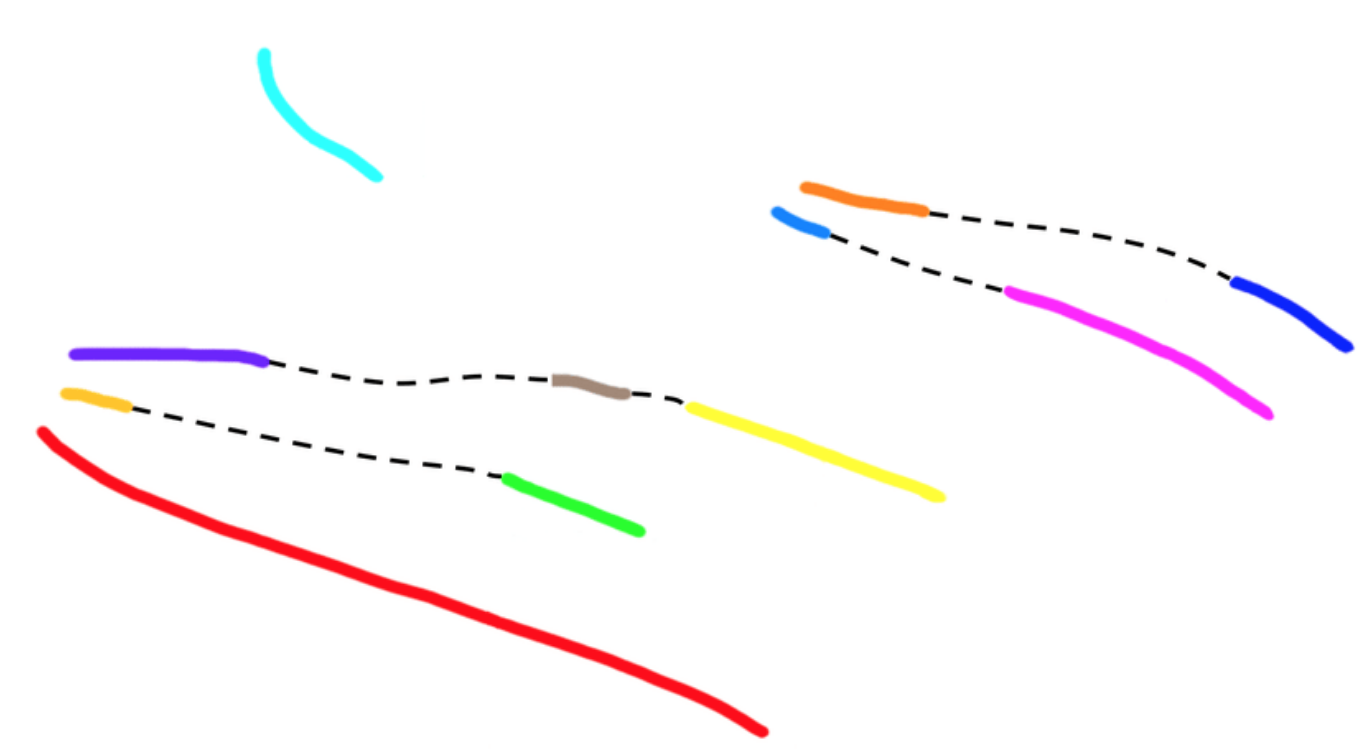
\includegraphics[width=100pt]{pics/fig9.png}
		\caption{Six objects with colors being diff. ids and dash lines being misses.}
	\end{figure}
		
	\vspace{-15pt}
	It's a drawback that trajectory matching only allows 1-1 relation.
	% Hence in the following, we have some quantities to measure
	% the overlapping of trajectories in the detection levels.
	% This aims to give some partial credits to non-matched good trackers.
			
\end{frame}

\begin{frame}
	\frametitle{Measures for Associations of Objects}
			
	By concepts in trajectory / id matchings,
	{\bf tracking associations of an single object} is developed in further.
	\emph{Do matching in detection levels and associate multiple ids by matching.}
	% {\color{red} Here the TP's, FP's and FN's are determined in framewise detection levels.}
			
	\vspace{4pt}
			
	Given a framewise matching $\Pi_\alpha$.
	Let $c = (g,p)$ be a TP pair in a frame $t$.
	We define TPA, FPA and FNA as follows.
	\begin{align*}
		\text{TPA}(c) :=                       
		\left\{(g_i, p_j)\in\text{TP}\ \left|\ 
		\begin{array}{c}                       
		\text{grId}(g_i)=\text{grId}(g),       \\
		\text{prId}(p_j) = \text{prId}(p)      
		\end{array}\right.                     
		\right\}.                              
	\end{align*}
	Note that $|\text{TPA}(c)|$ is just the number of frames that $\text{gtTraj}(g)$
	and $\text{prTraj}(p)$ overlap.
			
\end{frame}

\begin{frame}
	\frametitle{Measures for Associations of Objects}
			
	% Similarly, for the TP pair $c = (g, p)$, we also define the false positive associations
	% and false negative associations as follows.
	\vspace{-20pt}
	\begin{align*}
		\text{FPA}(c) := &             
		\left\{(g_i, p_j)\in\text{TP}\ \left|\ 
		\begin{array}{c}
		\text{grId}(g_i) \neq \text{grId}(g), \\
		\text{prId}(p_j) = \text{prId}(p)
		\end{array}\right.
		\right\} \\
		                 & ~ \bigcup ~ 
		\Big\{p_j\in\text{FP}\ |\ 
		\text{prId}(p_j) = \text{prId}(p)
		\Big\}; \\
		\text{FNA}(c) := &             
		\left\{(g_i, p_j)\in\text{TP}\ \left|\ 
		\begin{array}{c}
		\text{grId}(g_i) = \text{grId}(g), \\
		\text{prId}(p_j) \neq \text{prId}(p)
		\end{array}\right.
		\right\} \\
		                 & ~ \bigcup ~ 
		\Big\{g_i\in\text{FN}\ |\ 
		\text{gtId}(g_i) = \text{gtId}(g)
		\Big\}.
	\end{align*}
	Note that $\text{FPA}(c)$ and $\text{FNA}(c)$ relate to the non-matched or id-mismatched
	objects in $\text{prTraj}(p)$ and $\text{grTraj}(g)$.
		
	Later we'll see these terms in the definitions of HOTA metrics.
			
\end{frame}

\begin{frame}
	\frametitle{Measures for Associations of Objects}
	\begin{figure}
		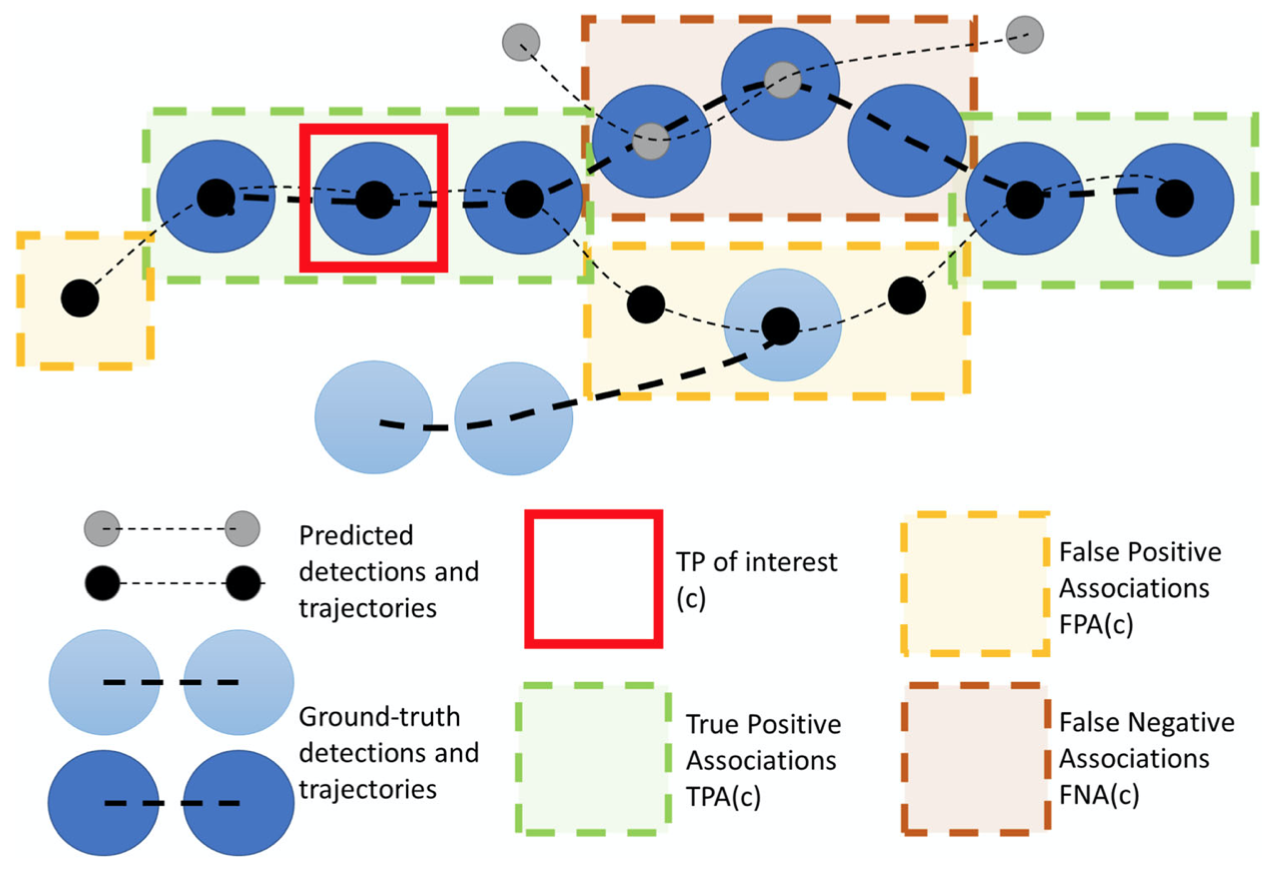
\includegraphics[width=220pt]{pics/fig8.png}
		\caption{For the interested object (red box), TPA: 5; FPA: 4; FNA: 3.}
	\end{figure}
\end{frame}

% \begin{frame}
%     In the next section,
%     we'll introduce metrics for measuring tracking results
%     via the defined quantities.

% \end{frame}

\section{Evaluation Metrics for Measuring Tracking Results}

\begin{frame}
	\frametitle{Metrics for Measuring Tracking Results}
			
	Performance of object trackings is based on the result of detections.
			
	\quad 
			
	To measure the results, metrics often consists of the following aspects
	\begin{itemize}
		\item detection;%: measure accuracies of predictions
		\item localization;%: measure accuracies of positions of correct predictions
		\item association.%: measure accuracies of the correct associations of objects
	\end{itemize}
			    
\end{frame}

\subsection{CLEAR-MOT: MOTA and MOTP}

\begin{frame}
	\frametitle{MOTA and MOTP}
			
	% {\scriptsize\tt K. Bernardin \& R. Stiefelhagen, Evaluating Multiple Object Tracking Performance:%
	% The CLEAR MOT Metrics.}
			
	Given a similarity threshold $\alpha$.
			
	\vspace{4pt}
			
	{\bf MOTA (multiple object tracking accuracy)} is calculated through
	\emph{optimizing the value}
	\[
		\text{MOTA}_\alpha :=
		\max_{\Pi_\alpha}
		\left\{1 - \dfrac{|\text{FN}_{\Pi_\alpha}| + |\text{FP}_{\Pi_\alpha}| + |\text{IDSW}_{\Pi_\alpha}|}{|\text{gtDet}|}\right\}
	\]
	among all matchings $\Pi_\alpha$ with $\mathcal S(c)\geq \alpha$ for all matched $c\in\Pi_\alpha$.
			
	\vspace{4pt}
			
	{\bf\color{blue} FN, FP terms affect the accuracy of detections.} \\
	{\bf\color{olive} The IDSW term affects the accuracy of id-associations.}
			
	\vspace{4pt}
		
	Remark: under $\alpha$, the matching is taken to optimize $|\text{TP}|$ as well.
			
\end{frame}

\begin{frame}
	\frametitle{CLEAR-MOT: MOTA and MOTP}
			
	As MOTA is achieved by some matching $\Pi_\alpha$, {\bf MOTP (multiple object tracking precision)}
	is calculated as follows:
	\[
		\text{MOTP}_\alpha =
		\dfrac{\sum_{(g,p)\in\text{TP}_{\Pi_\alpha}}\mathcal S(g,p)}{|\text{TP}_{\Pi_\alpha}|}.
	\]
	{\bf\color{red} MOTP measures the accuracy of localizations of predictions}.
			
	\vspace{4pt}
			
	By direct observations, if the MOTA value is low,
	then somehow it cannot be distinguished that
	the detections are not good or the tracking results are not good.
			
	\vspace{5pt}
		
	$\alpha\nearrow$ $\Rightarrow$ $|\text{FN}|, |\text{FP}|, \mathcal S \nearrow$, $|\text{TP}| \searrow$ $\Rightarrow$ MOTP $\nearrow$.
	$|\text{IDSW}|, \text{MOTA}$ $?$
		
			
			
\end{frame}

\subsection{Performance Measures for MTMCT: the ID Metrics}

\begin{frame}
	\frametitle{The ID Metrics}
			
	As a measure for the {\bf MTMCT (multi-target, multi-camera tracking)} tasks,
	the id metrics focus on matching of trajectories.
			
	\quad 
			
	Under a similarity threshold $\alpha$, the scoring functions are calculated through optimizing
	the quantity $|\text{IDTP}|$ by matching in sequence-levels as follows:
	\begin{align*}
		\text{ID-Precision} := & ~ \max_{\mathfrak P} \dfrac{|\text{IDTP}|}{|\text{IDTP}| + |\text{IDFP}|}, \\
		\text{ID-Recall} :=    & ~ \max_{\mathfrak P}\dfrac{|\text{IDTP}|}{|\text{IDTP}| + |\text{IDFN}|},  \\
		\text{IDF1} :=         &                                                                            
		~ \max_{\mathfrak P}\dfrac{|\text{IDTP}|}{|\text{IDTP}| + 0.5|\text{IDFP}| + 0.5|\text{IDFN}|}.
	\end{align*}
			
\end{frame}

\begin{frame}
	\frametitle{The ID Metrics}
			
	By direct observations, these id metrics show how good the whole tracking trajectories are.
	But once if several fragmentations occur in different frames,
	then we cannot not distinguish this case with the mostly lost cases.
			
	\begin{figure}
		\begin{subfigure}{.5\textwidth}
			\centering
			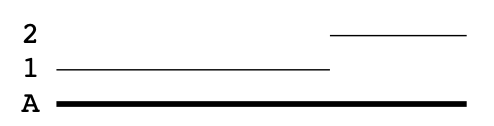
\includegraphics[width=120pt]{pics/fig6.png}
		\end{subfigure}%
		\begin{subfigure}{.5\textwidth}
			\centering
			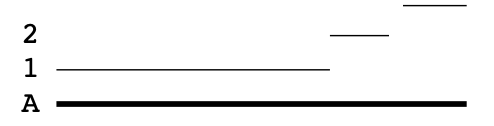
\includegraphics[width=120pt]{pics/fig7.png}
		\end{subfigure}
		\caption{The id metrics only measure tracking results of matched peices.
		The ground-truth id is shown by the bold line.}
	\end{figure}
			
\end{frame}

\subsection{Higher Order Tracking Accuracy: the HOTA metrics}

\begin{frame}
	\frametitle{The HOTA metrics}
		
	The HOTA score for a particular similarity threshold $\alpha$ is defined by
	optimizing the following value among matchings in detection levels:
	\[
		\text{HOTA}_\alpha := 
		\max_{\Pi_\alpha} \sqrt{\dfrac{\sum_{c\in\text{TP}} \mathcal A(c) }{|\text{TP}|+|\text{FN}|+|\text{FP}|}},
	\]
	where $\mathcal A(c)$ is the {\bf association score of a single pair of ids}:
	\[
		\mathcal A(c) = \dfrac{|\text{TPA}(c)|}{|\text{TPA}(c)|+|\text{FPA}(c)|+|\text{FNA}(c)|}.
	\]
	Note that the quantities TP, FP, FN, TPA, FPA, FNA also depend on matching $\Pi_\alpha$.
		
\end{frame}

\begin{frame}
	\frametitle{The HOTA metrics}
	The HOTA score is defined in a double Jaccard indices way.
	It can be divided into multiples of two values:
	Once the matching $\Pi$ is defined,
	\[
		\text{AssA}_\alpha = \dfrac{1}{|\text{TP}|} \sum_{c\in\text{TP}} \mathcal A(c), \ \ 
		\text{Det}_\alpha = \dfrac{|\text{TP}|}{|\text{TP}| + |\text{FP}| + |\text{FN}|}.
	\]
	Then we have the formula:
	\[
		\text{HOTA}_\alpha = \sqrt{\text{AssA}_\alpha \cdot \text{Det}_\alpha}.
	\]
	The two scores indicate the accuracy of tracking associations and the accuracy of detections.
\end{frame}

\begin{frame}
	\frametitle{The HOTA metrics}
		
	In the same time, by the same matching $\Pi_\alpha$,
	the localization score in HOTA is defined by
	\[
		\text{Loc}_\alpha = \dfrac{\sum_{c\in\text{TP}} \mathcal S(c)}{|\text{TP}|}.
	\]
	As a remark, $\text{AssA}_\alpha$ and $\text{Loc}_\alpha$ are not well-defined
	if $\text{TP} = \emptyset$.

	\vspace{4pt}

	Furthermore, the numerator can be changed to another metric for evaluating localizations
	(i.e. IoU, $\max\{1-\text{dist},0\}$, \ldots).
		
\end{frame}

\section{Implementation of HOTA metrics}

\subsection{Obtain the Optimization Matching}

\begin{frame}
	\frametitle{Matching to Optimize HOTA scores}
	
	The optimization is done by a Hungarian algorithm for
	\begin{itemize}
		\item maximizing the number of TP pairs as the first priority;
		\item and maximizing the mean of association scores
		      as a second objective across the set of maximized TP pairs.
	\end{itemize}
	
	To reduce time cost, this is fulfilled by the following scoring MS (match score) for
	potential matches between each ground-truth object and prediction:
	\[
		\text{MS}(i,j) =
		\begin{cases}
			1/\epsilon + \mathcal A_{\rm max}(i,j) + \epsilon\mathcal S(i,j), & \mathcal S(i,j) \geq \alpha; \\
			0,                                                                & \text{otherwise}.            
		\end{cases}
	\]
	
	\vspace{-5pt}
	$\mathcal A_{\rm max}$ is a `proxy' for $\mathcal A$ (association score).
	
\end{frame}

\begin{frame}
	\frametitle{Matching to Optimize HOTA scores}
	
	Since the values TPA's, FNA's and FPA's of a TP pair depend on matching in other frames,
	\emph{the optimizing matching can not be achieved by a linear assignment formulation}.
	
	\vspace{5pt}
	
	This value is a reference for the optimizing matching and is calculated as follows.
	\[
		\mathcal A_{\rm max}(c) = 
		\dfrac{|\text{TPA}_{\rm max}(c)|}{|\text{TPA}_{\rm max}(c)|+|\text{FNA}_{\rm min}(c)|+|\text{FPA}_{\rm min}(c)|}.
	\]
	Here the subscriptions mean to choose the possible maximum and minimum.
	But in the codes provided by author of the HOTA metrics, 
	they are just fractions like expectation values of matches.
	
\end{frame}

\subsection{The Algorithm Provided by the Author of HOTA metrics}

\begin{frame}
	\frametitle{The Official Calculation}
	\begin{figure}
		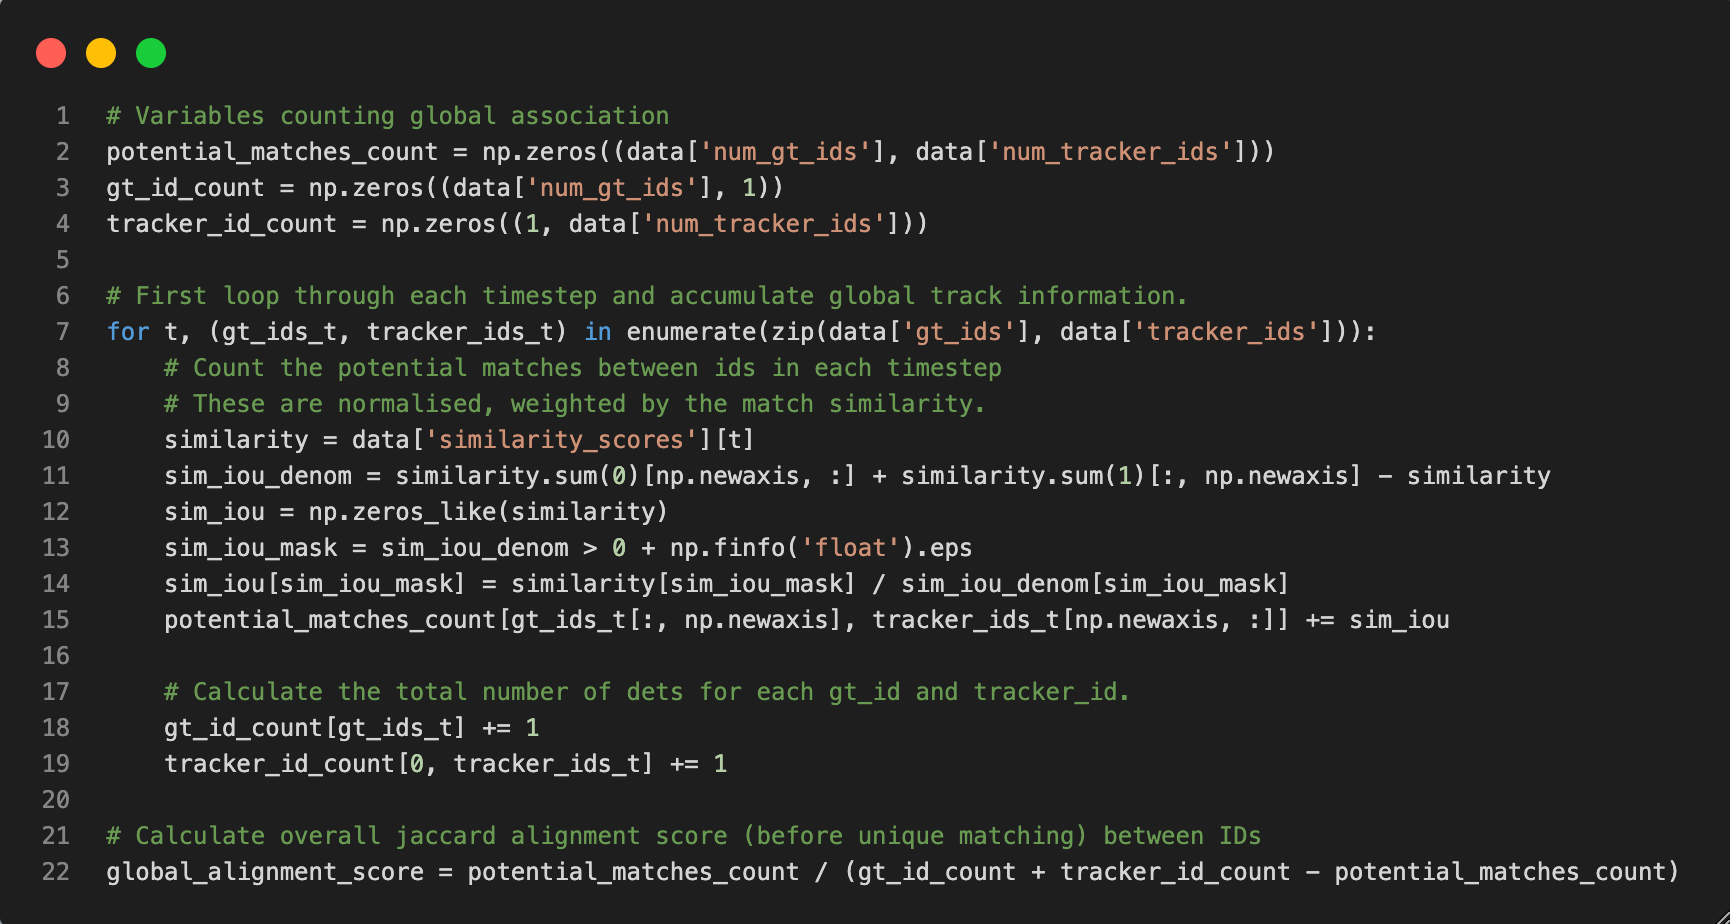
\includegraphics[width=280pt]{pics/fig10.png}
		\caption{Calculation of the proxies of association scores.}
	\end{figure}
\end{frame}

\begin{frame}
	\frametitle{The Official Calculation}
	\begin{itemize}
		\item IoU of similarities?
		      \begin{align*}
		      	\begin{bmatrix}	
		      	0.8                       & 0                       & 0.1                     \\
		      	0.5                       & 0.3                     & 0                       
		      	\end{bmatrix}
		      	\ \stackrel{\text{IoU}}{\Rightarrow}\ 
		      	\begin{bmatrix}
		      	\frac{0.8}{0.8+0+0.1+0.5} & 0                       & \frac{0.1}{0.8+0+0.1+0} \\
		      	\frac{0.5}{0.8+0.5+0.3+0} & \frac{0.3}{0+0.5+0.3+0} & 0                       
		      	\end{bmatrix} \\
		      	\text{(possible matches count $\approx$ TPA)}~ \Rightarrow ~ 
		      	\begin{bmatrix}
		      	4/7                       & 0                       & 1/9                     \\
		      	5/16                      & 3/8                     & 0                       
		      	\end{bmatrix}
		      \end{align*}
		\item Add this into {\scriptsize\tt `potential\_matches\_count'} according to indices.
		\item {\scriptsize\tt `gt\_id\_count'} and {\scriptsize\tt `track\_id\_count'} count
		      the numbers of frames that the ids appear. Their sum equals to $\text{FPA}+\text{FNA}+2\text{TPA}$.
		\item {\scriptsize\tt `global\_alignment\_score'}: the proxy value, approximation of $\mathcal A$.
		      		
	\end{itemize}
\end{frame}

\begin{frame}
	\frametitle{The Official Calculation}
	\begin{figure}
		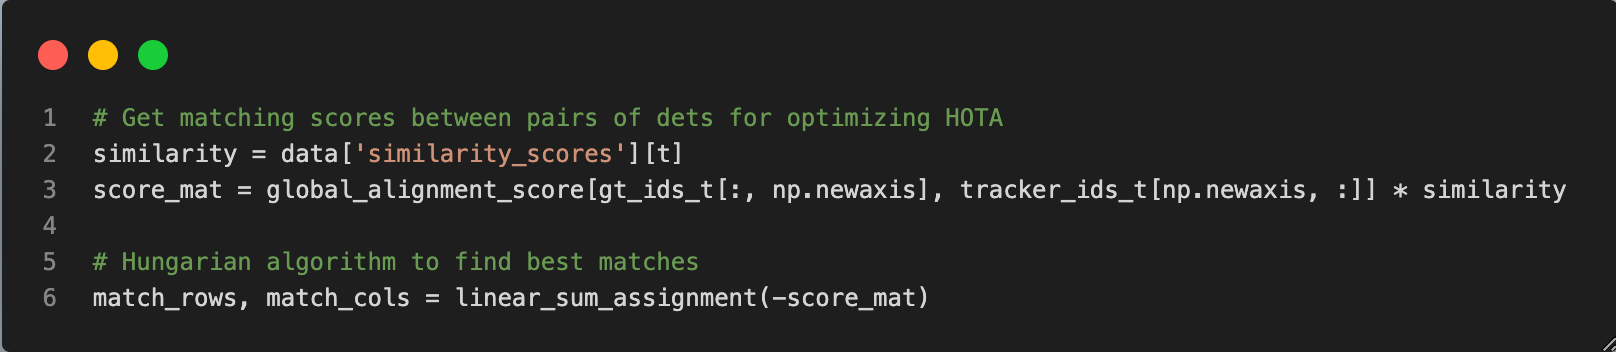
\includegraphics[width=280pt]{pics/fig11.png}
		\caption{Perform matching by optimizing the proxy score weighted
			by the local similarity via a Hungarian algorithm.}
	\end{figure}

	\vspace{-15pt}

	Then calculate the association scores by the `actual matching'.

	\vspace{3pt}

	By given similarity threshold $\alpha$,
	\begin{itemize}
	\item filter out matched pairs whose similarities less than $\alpha$;
	\item calculate the $\text{HOTA}_\alpha$ score; and
	\item calculate the $\text{LocA}_\alpha$ score.
	\end{itemize}

\end{frame}

\begin{frame}
	\frametitle{The Official Calculation: the Integration of HOTA scores}

	Besides of the localization score $\text{LocA}_\alpha$,
	integration of $\text{HOTA}_\alpha$ scores in different $\alpha$'s
	could also measure the performance of localization.
	This integration can be approximated by evaluating $\text{HOTA}_\alpha$
	for $\alpha$'s that partitions $[0,1]$.
	That is,
	\[
		\int_0^1 \text{HOTA}_\alpha~ d\alpha ~ \approx ~ \dfrac{1}{19}\sum_{\alpha\in A} \text{HOTA}_\alpha
	\]
	where $A:=\{0.05, 0.1, 0.15, \cdots, 0.9, 0.95\}$.

\end{frame}

\subsection{Implementation in linker-metrics}

\begin{frame}
	\frametitle{Recall the Road Map of linker-metrics}

	\begin{figure}
		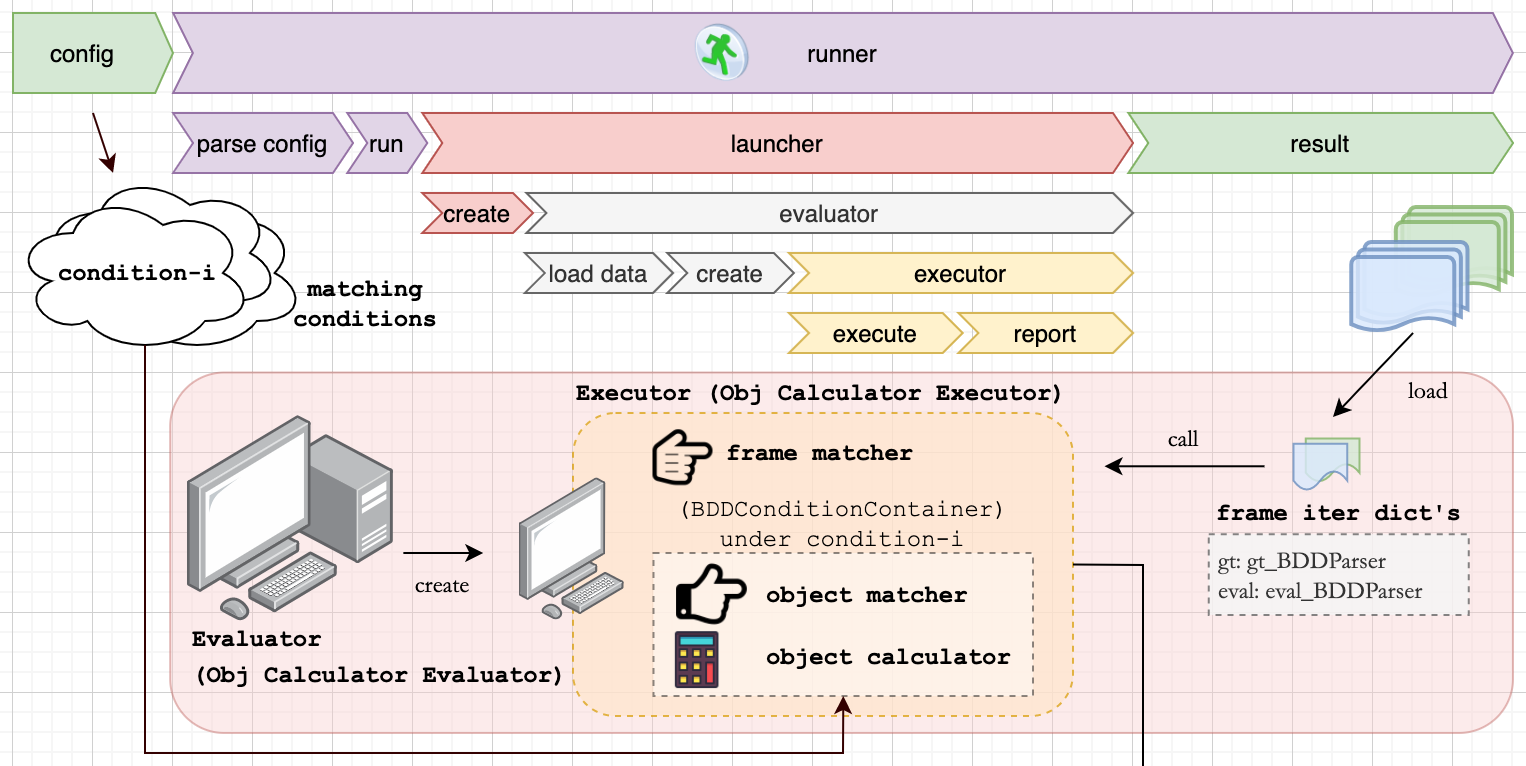
\includegraphics[width=300pt]{pics/fig12.png}
		\caption{runner $\to$ launcher $\to$ evaluator (calculation executor).}
	\end{figure}
\end{frame}

\begin{frame}
	\frametitle{Processing in linker-metrics}

	\begin{figure}
		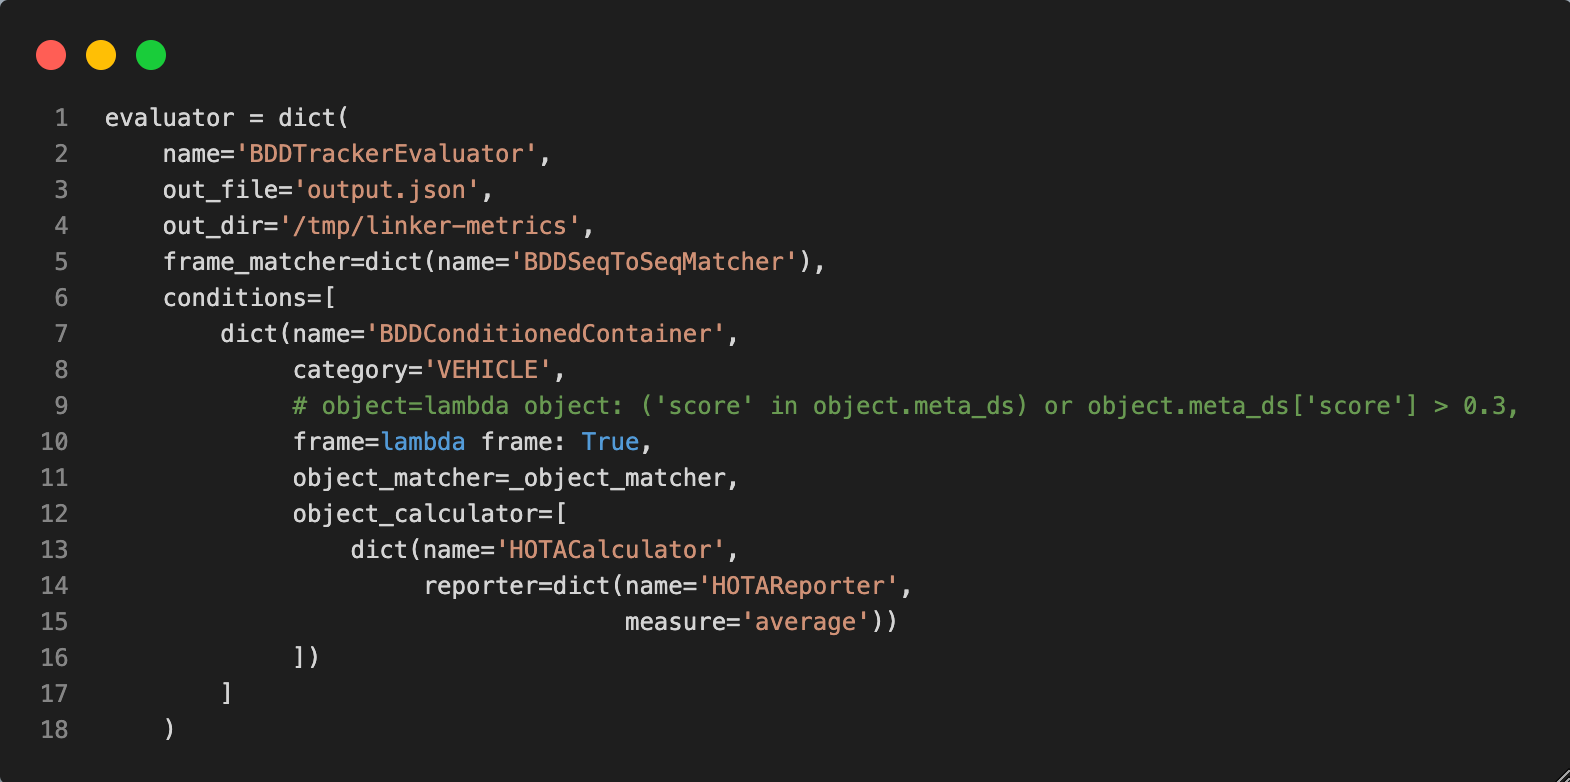
\includegraphics[width=280pt]{pics/fig13.png}
		\caption{linker-metrics uses config file to control the evaluation process.}
	\end{figure}

\end{frame}

\begin{frame}
	\frametitle{Calculation for HOTA scores}

	Each step in calculation of HOTA scores is performed by frame matcher, object matcher
	and object calculator in linker-metrics.

	\begin{itemize}
	\item The {\tt sequence-to-sequence matcher} parses the matched data sequentially.

	\item The object matcher {\tt sequential instances matcher} calculate the proxies
		during a `pre-match' performed by the build-in pre-matcher (here uses {\tt IoU matcher}).

	\item Then the object calculator {\tt HOTACalculator} calculate the HOTA scores
		according to the actual matching returned by object matcher.
	\end{itemize}

\end{frame}

\begin{frame}
	\frametitle{}
\end{frame}

\end{document}